% !TEX root = ../main.tex
\section{实验\chinese{section}}
\subsection{实验题目}
ADC12实验
\subsection{实验目的}
ADC12单次采样A0端口,根据转换结果控制LED状态。
参考时钟源MODOSC(缺省),参考电压AVcc(缺省),SAMPCON信号来自采样定时器,ADC12MEMO8作为转换地址。若A0 < 0.5*AVcc,点亮P4.1口LED,A0 > 0.5*AVcc,点亮P4.2口LED。
\subsection{实验仪器和设备}计算机、开发板、示波器、信号源、电源、Code Composer Studio v5、串口调试助手等。
\subsection{实验步骤}
\begin{lstlisting}[language=C]
/****************************************
       |            P4.3|--> LED_Red
     --|RST         P4.2|--> LED_Green
Vin -->|P6.0/CB0/A0 P4.1|--> LED_Yellow
****************************************/
\end{lstlisting}
\par\indent 关闭看门狗,设置ADC12模块,包括ADC12的时钟系统、控制信号、转换位置等。开总中断和ADC12MEM8中断,单次单通道转换,转换完成后会发生一次中断,在中断处理函数中读取数值并通过LED等显示出来。
\subsection{程序清单}
\lstinputlisting{src/code/ADC12.c}
\subsection{实验结果记录与分析}
\begin{figure}[htbp]
	\centering
	\begin{minipage}[htbp]{7.5cm}
		\centering
		\caption{ADC12,低电位}
		\label{ADC121}
		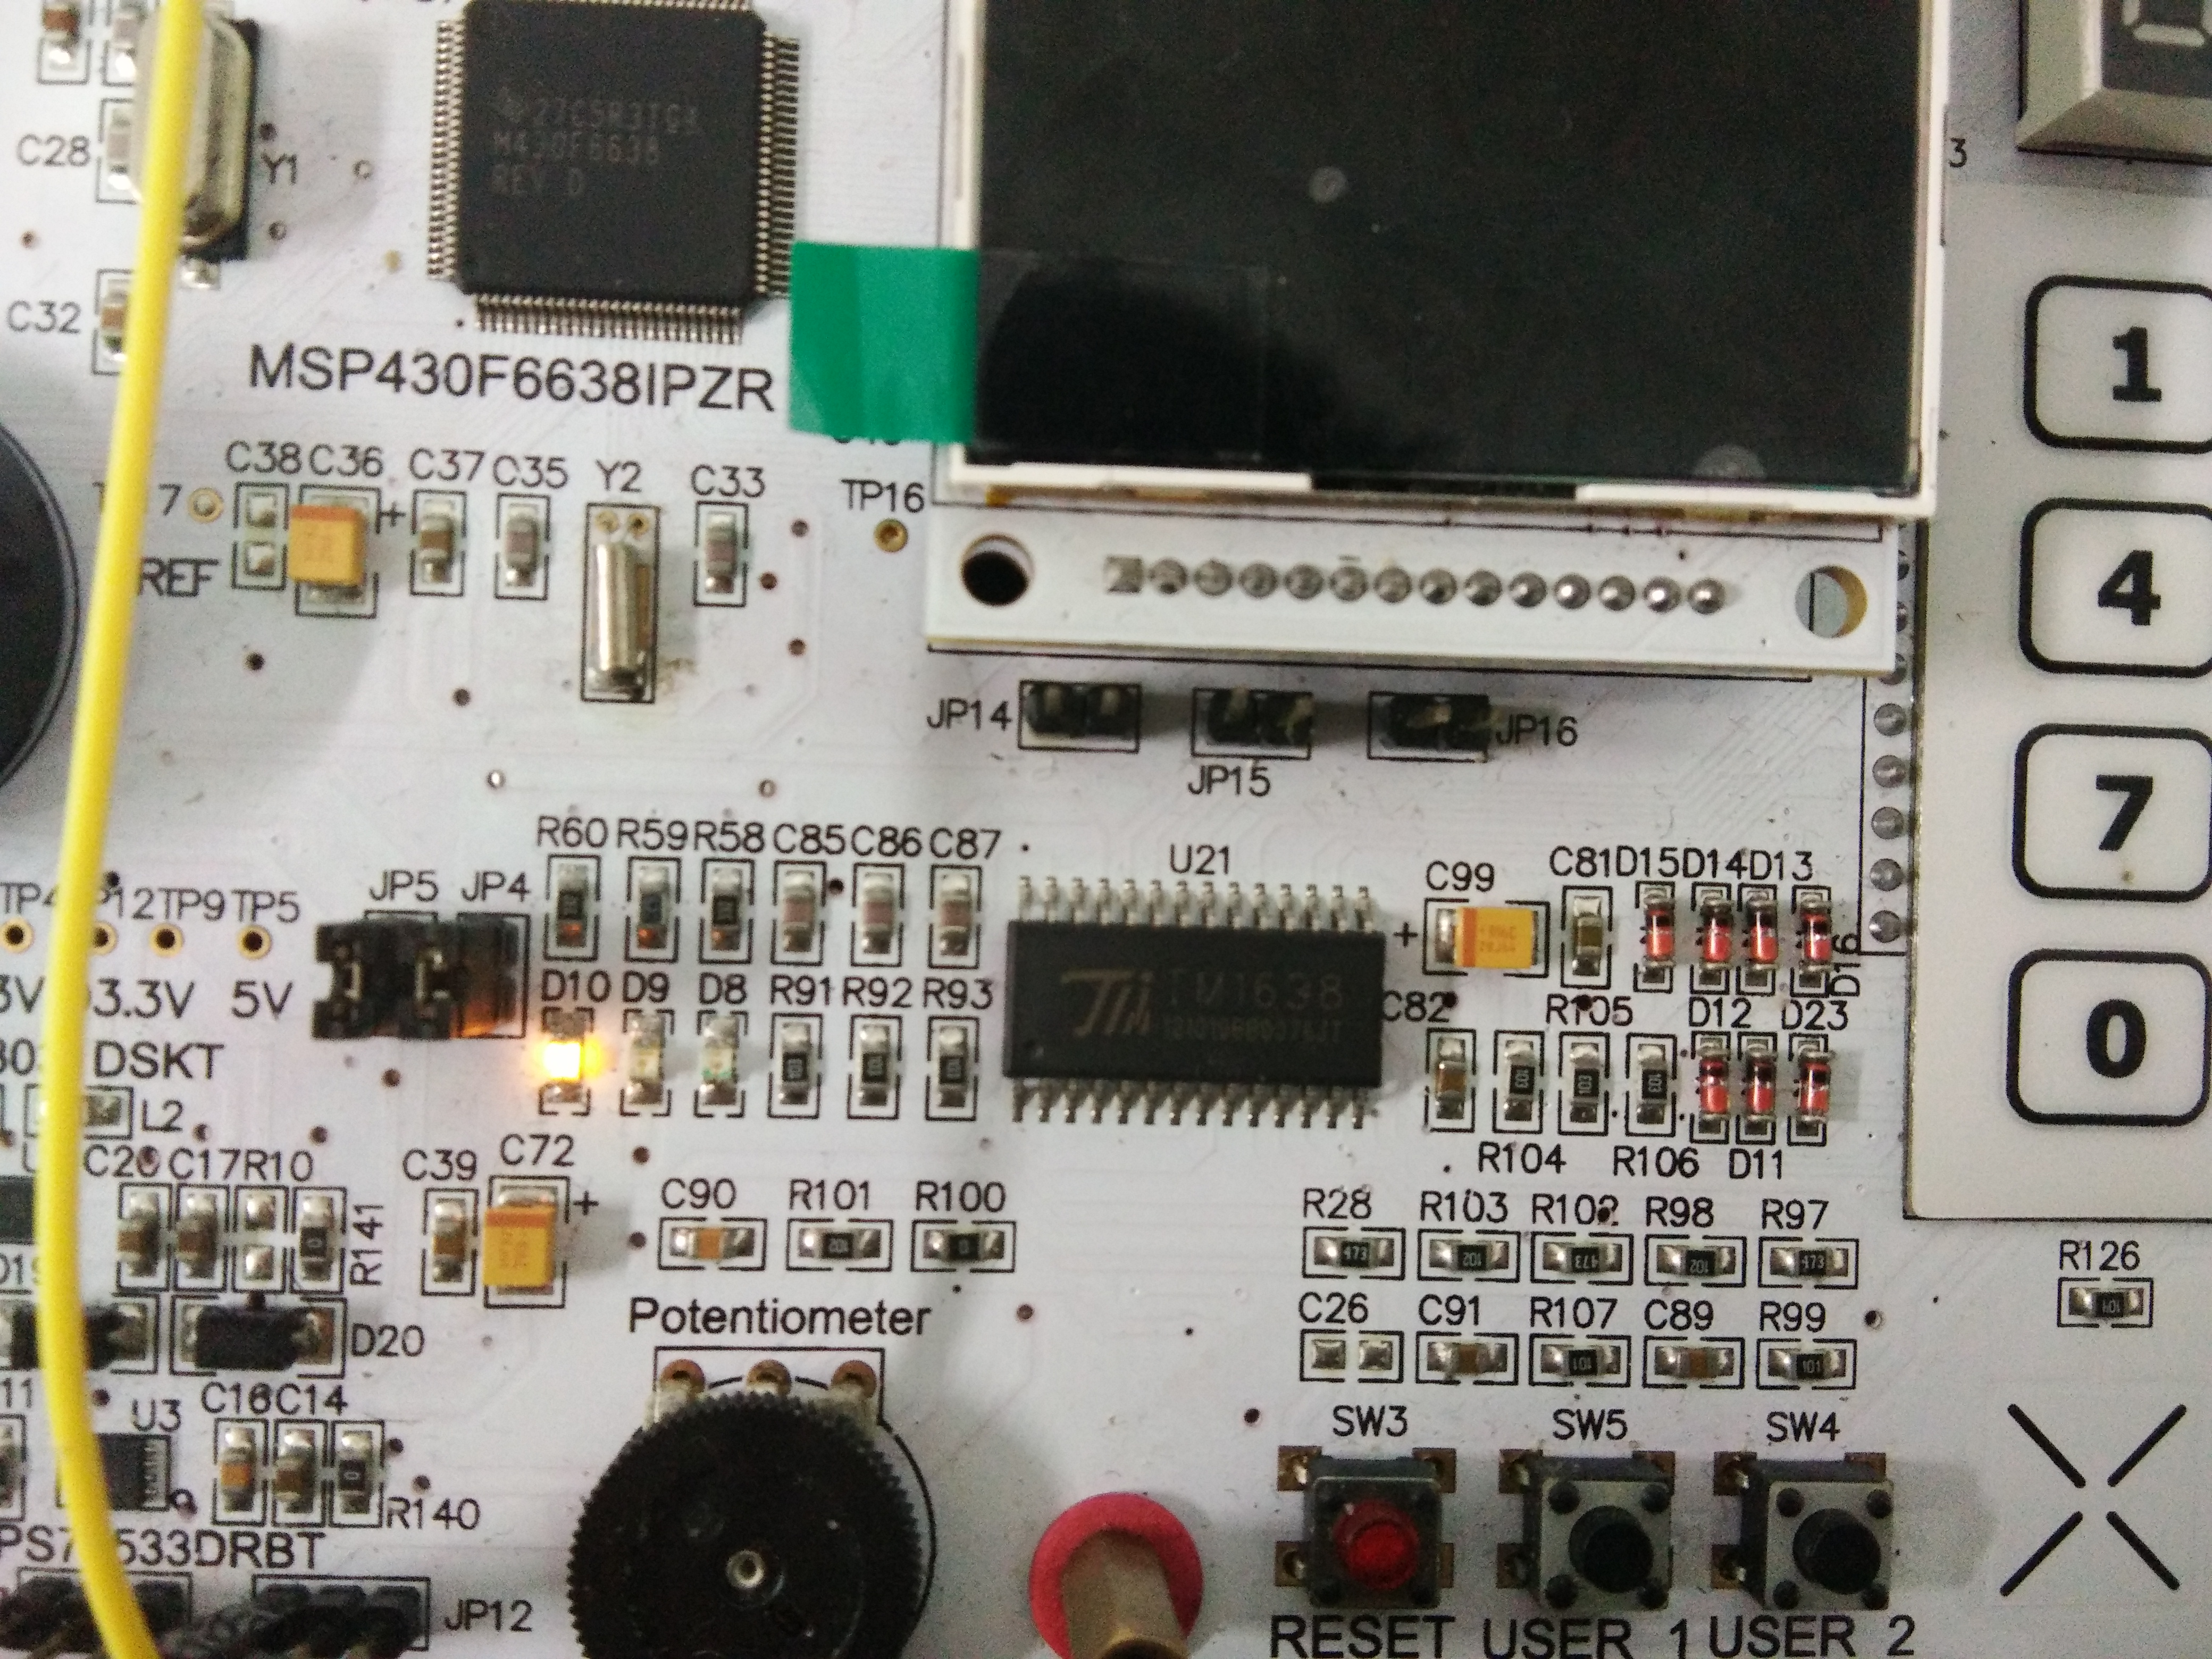
\includegraphics[width=7.5cm]{bitmap/jpg/ADC121.jpg}
	\end{minipage}
	\begin{minipage}[htbp]{7.5cm}
		\centering
		\caption{ADC12,高电位}
		\label{ADC122}
		\includegraphics[width=7.5cm]{bitmap/jpg/ADC122.jpg}
	\end{minipage}
\end{figure}
\subsection{遇到的问题与解决方法}
\begin{enumerate}
	\item 实验箱有故障,而且不止一个实验箱有故障。无论怎么调电位器LED灯都只显示电压最小的情况。调试后发现接线、电位器都是好的,但一旦跟P6.0连接后就会恒为低电压。如果将P6.0触接5V,灯会立刻全闪然后全灭。触接DVCC也是一样。换了1个实验箱就好了。这大概就是常说的软件有问题先查硬件吧。
\end{enumerate}
